\documentclass{article}

\usepackage{physics} % Handy shortcuts like \pdv, \dd and much more
\usepackage{geometry} % smaller margins, can be adjusted if given arguments
\usepackage{siunitx} % the \si environment for units
\usepackage{mathtools} % The dcases environment, prettier than just cases
\usepackage{tikz} % For drawing picures
\usepackage{wrapfig} % Wrapping text around figures
\usepackage{enumitem} % Getting alphabetical enumerate


\title{Exercise 8 - TFY4345 Classical Mechanics}
\date{2020}

\begin{document}
    \maketitle
    \section{Principal moments of inertia of a triangular slab}
    \begin{wrapfigure}{r}{0.4\textwidth}
        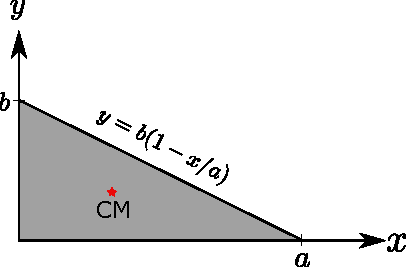
\includegraphics[width=0.4\textwidth]{figures/exercise_1_triangle.pdf}
        % \vspace{-3cm}
    \end{wrapfigure}\leavevmode
    (Exam Aug. 2019) \\
    \begin{enumerate}[label=(\alph*)]
        \item Compute the center-of-mass (CM) for the planar triangle in the figure, assuming it to be of uniform two-dimensional mass density $\rho$.
        \item Compute the inertia tensor \emph{with respect to the origin,} for the same triangle.
        \item (Optional) If the origin is shifted to the CM, the inertia tensor becomes (this can be show by using the Steiner's parallel axis theorem)
        \begin{equation*}
            I_{CM} = 
            \begin{pmatrix*}
                I_{11} & I_{12} & 0 \\
                I_{21} & I_{22} & 0 \\
                0 & 0 & I_{33} \\
            \end{pmatrix*}
             =\frac{M}{18} 
            \begin{pmatrix*}
                a^2 & \frac{1}{2}ab & 0 \\
                \frac{1}{2}ab & b^2 & 0 \\
                0 & 0 & a^2 + b^2 \\
            \end{pmatrix*}
        \end{equation*}
        where $I_{xy} = I_{yx}$ and $I_{xx} + I_{yy} = I_{zz}$ in the general form show first. Define next
        \begin{equation*}
            A = \frac{1}{2}(I_{xx} + I_{yy}), \quad B = \sqrt{\frac{1}{2}(I_{xx} - I_{yy})^2 + I_{xy}^2}, \quad \vartheta = \tan^{-1}\bigg( \frac{2I_{xy}}{I_{xx} - I_{yy}}\bigg).
        \end{equation*}
        Derive the principal moments of inertia and the principal axes by using the general form of the inertia tensor, and these new variables.
    \end{enumerate}
    [Hint] The last equations comprises a relationship that can be described by a right triangle.
    \newpage
    \begin{wrapfigure}{r}{0.55\textwidth}
        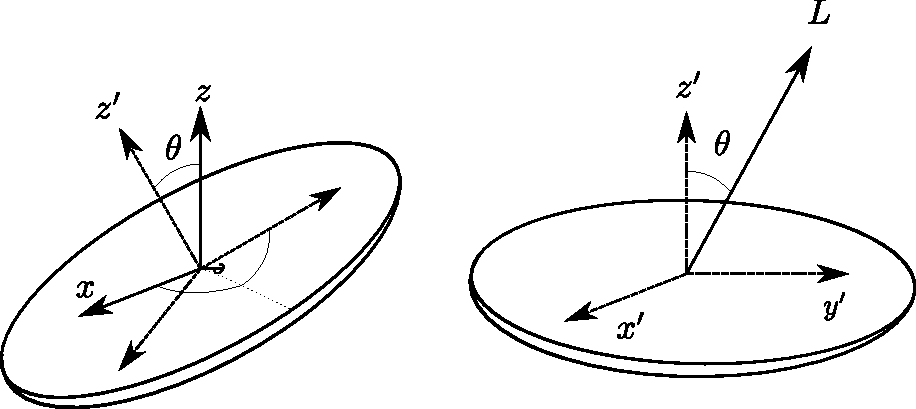
\includegraphics[width=0.55\textwidth]{figures/exercise_2_frisbee.pdf}
        \vspace{-2cm}
    \end{wrapfigure}\leavevmode % Horrible hack
    \section{Precession of a frisbee}

    (Exam Aug. 2016) \\ \\
    Consider an axial-symmetric body with the principal moments of inertia $I_1 = I_2 \neq I_3$ for rotation around the axis of symmetry. The angular momentum in the laboratory frame is $\mathbf{L} = L \mathbf{e}_z$, where $z$ is the symmetry axis. 
    \begin{enumerate}[label=(\alph*)]
        \item Derive the equations of motion for the body, using the Euler equations and the angles $\theta, \psi$ and $\phi$. Define also the components of $\boldsymbol{\omega}$. (See lecture notes, we derived this already!)
        \item Find the expression for the Euler angles $\theta, \psi, \phi$ as a function of time.
        \item Assume $I_3 = 2I_1$. The precession (wobble) of the frisbee is given by $\dot \phi$. Show that the precession is twice as fast as the rotation frequency of the frisbee, assuming that $\theta$ is small (i.e. that $\cos(\theta) \approx 1$).
    \end{enumerate}

    \section{Precession of a heavy spinning top}
    (Based on example p. 208-223 in Goldstein 3rd. ed., p. 70-74 in the compendium)\\ \\
    In the example we define the shifted energy as 
    \begin{equation*}
        E' = \frac{1}{2}I_1 \dot \theta^2 + V(\theta), \quad V(\theta) = \frac{(p_\phi - p_\psi \cos(\theta)^2)}{2I_1\sin(\theta)^2} + Mgh\cos(\theta),
    \end{equation*}
    which is a constant of motion. We also defined $\theta_0$ to be the constant angle of inclination of spinning top with regular precession, e.g. that the symmetry axis rotates around the $z$ at a fixed angle. Consider the shape of the effective potential $V(\theta)$ for $\theta_0$. \emph{What is the condition in this case?} The following change of variables will come in handy for the result:
    \begin{equation*}
        \beta = p_\phi - p_\psi \cos(\theta_0).
    \end{equation*}
    You will encounter a quadratic equation for $\beta$. Show that for the equilibrium precession inclination angle $\theta_0$, the following must hold true:
    \begin{equation*}
        \omega_3 \le \frac{2}{I_3}\sqrt{MghI_1 \cos(\theta_0) }.
    \end{equation*}
    What can you say about the corresponding precession angular velocity $\dot \phi_0$?




\end{document}
